\documentclass[tikz,border=10pt]{standalone}
\usepackage{tikz}
\usepackage{amsmath}
\usetikzlibrary{decorations.pathreplacing}

\begin{document}

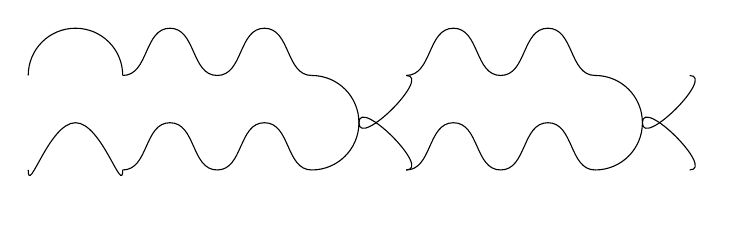
\begin{tikzpicture}[scale=1.2]
    % First saddle move
    \draw (0,0) to[out=90,in=180] (0.5,0.5) to[out=0,in=90] (1,0);
    \draw (0,-1) to[out=-90,in=180] (0.5,-0.5) to[out=0,in=-90] (1,-1);
    
    % First twist region
    \draw (1,0) to[out=0,in=180] (1.5,0.5) to[out=0,in=180] (2,0) 
          to[out=0,in=180] (2.5,0.5) to[out=0,in=180] (3,0);
    \draw (1,-1) to[out=0,in=180] (1.5,-0.5) to[out=0,in=180] (2,-1) 
          to[out=0,in=180] (2.5,-0.5) to[out=0,in=180] (3,-1);

    % Second saddle move
    \draw (3,0) to[out=0,in=90] (3.5,-0.5) to[out=-90,in=0] (4,0);
    \draw (3,-1) to[out=0,in=-90] (3.5,-0.5) to[out=90,in=0] (4,-1);

    % Second twist region
    \draw (4,0) to[out=0,in=180] (4.5,0.5) to[out=0,in=180] (5,0) 
          to[out=0,in=180] (5.5,0.5) to[out=0,in=180] (6,0);
    \draw (4,-1) to[out=0,in=180] (4.5,-0.5) to[out=0,in=180] (5,-1) 
          to[out=0,in=180] (5.5,-0.5) to[out=0,in=180] (6,-1);

    % Third saddle move
    \draw (6,0) to[out=0,in=90] (6.5,-0.5) to[out=-90,in=0] (7,0);
    \draw (6,-1) to[out=0,in=-90] (6.5,-0.5) to[out=90,in=0] (7,-1);
    
\end{tikzpicture}

\end{document}